%! TEX root = ../main.tex
\documentclass[main]{subfiles}

\begin{document}
\section{表面繊維の調査}

カーリングブラシパッドの表面性状を,特に使用回数に伴い,どれだけ摩耗しているかを
デジタルマイクロスコープを用いて観察した.デジタルマイクロスコープは,光学系とデジタルカメラを組み合わせた
高性能な顕微鏡の一種である.対象物を光学的に拡大して観察することができ,対象物からの光をデジタルセンサーに
取り込む.内蔵の画像処理技術により,高解像度の画像を生成する.本研究では100倍~1000倍まで見ることができる
デジタルマイクロスコープを使用した.それぞれのサンプルで、一番汚れている箇所(\ref{fig:sample1}の赤枠)と
汚れが少ない箇所(\ref{fig:sample1}の黒枠)を撮影した.10~15投使用したものと長期間使用したものはサンプル
を2つずつ用意した.肉眼で観察した際に長期間使用したものはそれぞれのサンプルで大きな違いは見られなかった.
しかし10~15投使用したものに関して,本研究で使用したカーリングブラシパッドは,汚れ具合から左右偏りなく使用
されているもの(\ref{fig:labelB})と片方に使用具合が偏っているもの(\ref{fig:labelC})があった.
具体的には下記の項目どおりである.

\begin{itemize}
    \item 未使用×1
    \item 10~15投使用×2
    \item 長期間使用×2
\end{itemize}

\begin{figure}[htbp]
    \centering
    \begin{subfigure}[htbp]{0.3\linewidth}
        \centering
        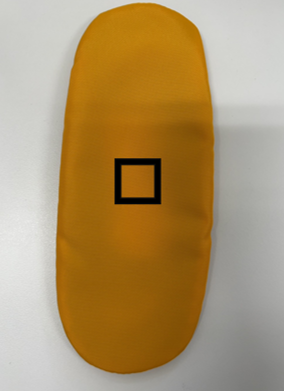
\includegraphics[keepaspectratio, width=0.8\linewidth, height=\linewidth]{figures/caring_brush_pad/misiyou.png}
        \caption{未使用}
        \label{fig:labelA}
    \end{subfigure}
    \begin{subfigure}[htbp]{0.3\linewidth}
        \centering
        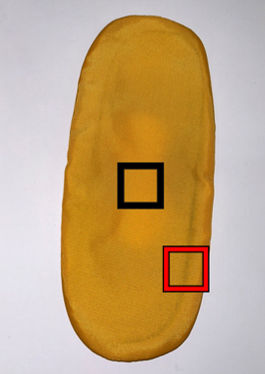
\includegraphics[keepaspectratio, width=0.8\linewidth, height=\linewidth]{figures/caring_brush_pad/10~15A.png}
        \caption{10~15投使用A}
        \label{fig:labelB}
    \end{subfigure}
    \begin{subfigure}[htbp]{0.3\linewidth}
        \centering
        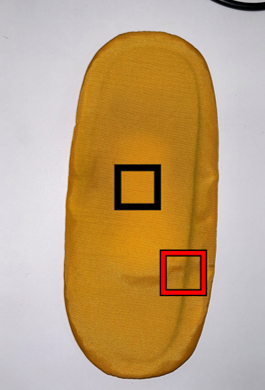
\includegraphics[keepaspectratio, width=0.8\linewidth, height=\linewidth]{figures/caring_brush_pad/10~15B.png}
        \caption{10~15投使用B}
        \label{fig:labelC}
    \end{subfigure}
    \begin{subfigure}[htbp]{0.3\linewidth}
        \centering
        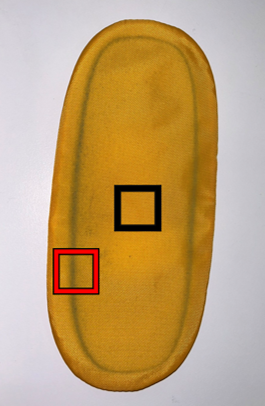
\includegraphics[keepaspectratio, width=0.8\linewidth, height=\linewidth]{figures/caring_brush_pad/chouki.png}
        \caption{長期間使用A}
        \label{fig:labelD}
    \end{subfigure}
    \begin{subfigure}[htbp]{0.3\linewidth}
        \centering
        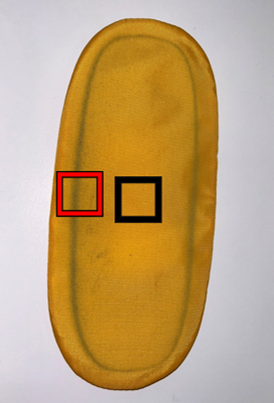
\includegraphics[keepaspectratio, width=0.8\linewidth, height=\linewidth]{figures/caring_brush_pad/choukiB.png}
        \caption{長期間使用B}
        \label{fig:labelE}
    \end{subfigure}
    \caption{カーリングブラシパッド}
    \label{fig:sample1}
\end{figure}


\end{document}